\begin{figure}[h]
    \centering
    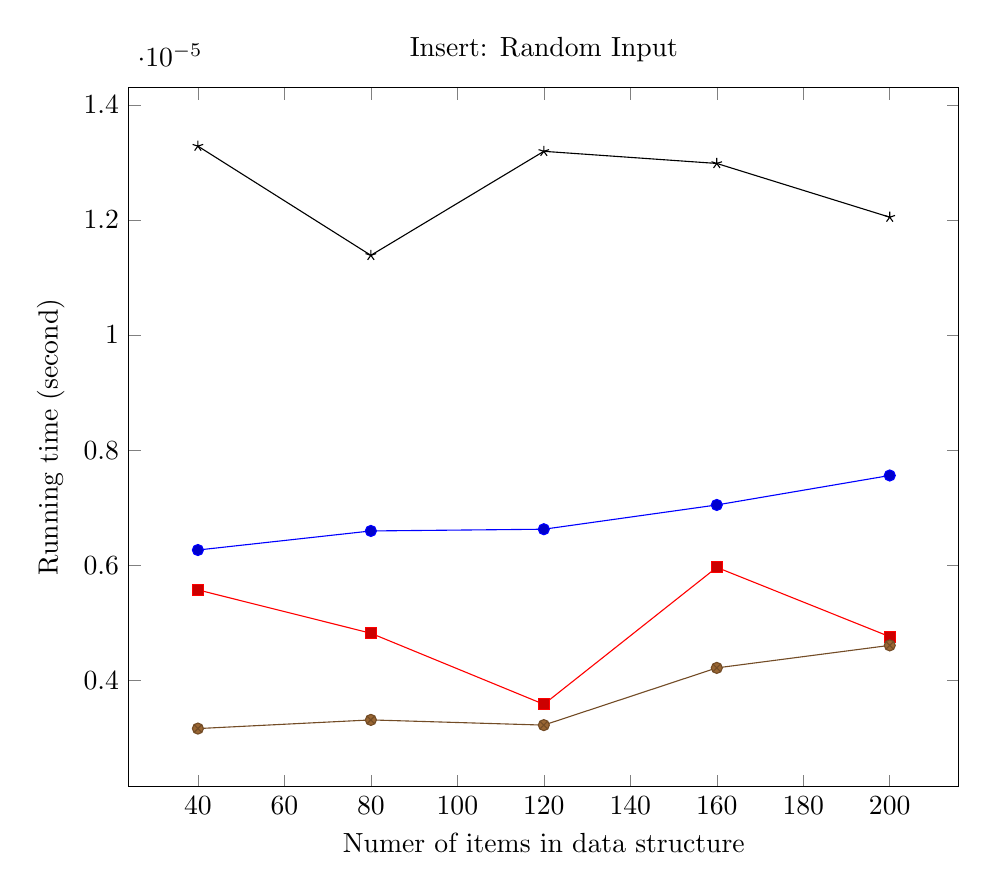
\begin{tikzpicture}
        \begin{axis}[
            xlabel={Numer of items in data structure},
            ylabel={Running time (second)},
            title={Insert: Random Input},
            width=\textwidth
        ]
		\addplot coordinates {
			(200, 7.559500952469822e-06)
			(160, 7.047502879986567e-06)
			(120, 6.625857408537605e-06)
			(80, 6.595739874859508e-06)
			(40, 6.264447004439289e-06)
		};
		\addplot coordinates {
			(200, 4.758570320678724e-06)
			(160, 5.963271667680514e-06)
			(120, 3.583986507343928e-06)
			(80, 4.818805388023817e-06)
			(40, 5.571743729909651e-06)
		};
		\addplot coordinates {
			(200, 4.607982652299336e-06)
			(160, 4.216454714522922e-06)
			(120, 3.2225761032400602e-06)
			(80, 3.3129287042688025e-06)
			(40, 3.1623410358894156e-06)
		};
		\addplot coordinates {
			(200, 1.2047013470067868e-05)
			(160, 1.2980657013994534e-05)
			(120, 1.3191479749724565e-05)
			(80, 1.1384427729210777e-05)
			(40, 1.3281832350747758e-05)
		};
        \legend{}
        \end{axis}
    \end{tikzpicture}
    \caption{Average of 0 operations, benchmarked every 0, starting at 0.}
\end{figure}